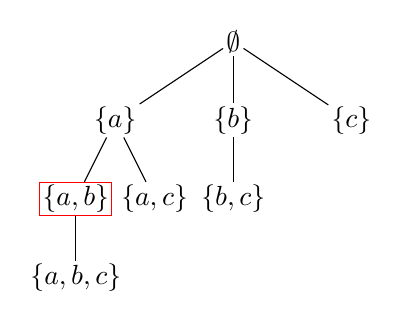
\begin{tikzpicture}[every node/.style={inner sep=1pt}]
  % Level 0
  \node (empty) at (2,0) {$\emptyset$};
  % Level 1
  \node (a) at (0.5,-1) {$\{a\}$};
  \node (b) at (2,-1) {$\{b\}$};
  \node (c) at (3.5,-1) {$\{c\}$};
  % Level 2
  \node[draw=red, label=left:{\xmark}] (ab) at (0,-2) {$\{a,b\}$};
  \node (ac) at (1,-2) {$\{a,c\}$};
  \node (bc) at (2,-2) {$\{b,c\}$};
  % % Level 3
  \node (abc) at (0,-3) {$\{a,b,c\}$};
  Edges
  \draw (empty) -- (a);
  \draw (a) -- (ab);
  \draw (ab) -- (abc);
  \draw (a) -- (ac);

  \draw (empty) -- (b);
  \draw (b) -- (bc);
  \draw (empty) -- (c);
\end{tikzpicture}

%%% Local Variables:
%%% mode: latex
%%% TeX-master: "../main"
%%% End: